\documentclass[10pt]{beamer}
\usepackage[utf8]{inputenc}
\usepackage[croatian]{babel}
\usepackage{graphicx}
\usetheme{Bergen}

\usepackage{amsfonts}
\usepackage{amssymb}
\usepackage{graphicx}
\usepackage{url}
%\usepackage{wrapfig}
%\usepackage[table]{xcolor}
%\definecolor{lightgray}{gray}{0.9}
%\usepackage[hidelinks]{hyperref}
%\usepackage{subcaption}
%\usepackage{float}
%\usepackage{listings}
\usepackage{pgfplots}
%\usepackage{cite}
\begin{document}
	\author{Matea Novak \and Filip Novački}
	\title{Linearni splajn i po dijelovima kubična interpolacija}
	\subtitle{Odabrana poglavlja matematike}
	%\logo{}
	\institute{}
	%\date{}

	%\setbeamercovered{transparent}
	%\setbeamertemplate{navigation symbols}{}
	\begin{frame}[plain]
	\maketitle
\end{frame}
\tableofcontents
\section{Uvod}
\begin{frame}{Uvod}

\end{frame}
\section{Glavna ideja}
	\begin{frame}{Glavna ideja}
		\begin{itemize}
			\item[Motivacija ] Predviđanje vrijednosti između dviju izmjerenih diskretnih vrijednosti
			\pause
			\item[Tipovi interpolacija: ] 
			\item[Linearna ] Svojstva:
			\begin{itemize}
				\item Jednostavna za računati
				\item Nije uvijek dovoljno precizna
			\end{itemize}
		
			\item[Kvadratna ] Svojstva:
			\begin{itemize}
				\item Nema fizikalne podloge
				\item Kontrola derivacije nedovoljno dobra
			\end{itemize}
			\item[Kubična ] Svojstva:
			\begin{itemize}
				\item Glatka (neprekidna u čvorovima)
				\item Relativno precizna
				\item Dovoljno jednostavna za računati
			\end{itemize}
			\item[Višeg reda ] Svojstva:
			\begin{itemize}
				\item Teške za računati
				\item Imaju tendenciju divljati u ekstremnim točkama
			\end{itemize}
		\end{itemize}
	\end{frame}
\section{Algoritmi}
\subsection{Linearna interpolacija}
\begin{frame}{Algoritam za linearnu interpolaciju}
	\begin{alertblock}{Zadavanje zadataka:}
		\begin{equation*}
		x_i=a+ih,\quad i=0,1,\ldots,n,\quad h=\frac{b-a}{n}
		\end{equation*}
	\end{alertblock}

	\begin{alertblock}{Pravac između čvorova za $x_i$ i $x_{i+1}$}
		\begin{equation}
		y=\biggr{(}\frac{y_{i+1}-y_i}{x_{i+1}-x_i}\biggr{)}(x-x_i)+y_i
		\label{pravac}
		\end{equation}
	\end{alertblock}

	
\end{frame}
\begin{frame}{Primjer izračuna}
	\begin{exampleblock}{Čvor za točku u $x=0$, funkcija $f(x)=\sin x$}
		\begin{align*}
		x_0=&0\quad\rightarrow \quad y_0=f(0)=0\\
		x_1=&a+ih\\=&0+1\frac{2\pi-0}{40}\\
		=&0.15707963267948966\\
		y_1=&f\biggr{(}\frac{2\pi}{40}\biggr{)}\\=&0.15643446504023087
		\end{align*}
	\end{exampleblock}
	\begin{exampleblock}{Interpolacijski pravac}
		\begin{equation}
		y=1.0041242039539873x
		\label{linInt1}
		\end{equation}
	\end{exampleblock}
\end{frame}
\subsection{Kubična interpolacija}
\begin{frame}{Algoritam za kubičnu interpolaciju}

	\begin{exampleblock}{Zadavanje zadataka}
		\begin{equation*}
		x_i=a+ih,\quad i=0,1,\ldots,n,\quad h=\frac{b-a}{n}
		\end{equation*}
	\end{exampleblock}
	\begin{exampleblock}{Računanje $C$}
		\begin{equation*}
		C_{k, i}=\frac{f^{i'}(x_0)}{i!},\quad k\in [0, 3]
		\end{equation*}
		
	\end{exampleblock}
	
	\begin{exampleblock}{Hermitova jednadžba polinoma}
	\begin{align*}
	P_i(x)=&C_{0,i}+\\&C_{1,i}(x-x_{i-1})+\\&C_{2,i}(x-x_{i-1})^2+\\&C_{3,i}(x-x_{i-1})^3 \\
	x\in[&x_{i-1}, x_i], i=1,...,n
	\end{align*}	
	\end{exampleblock}
	
\end{frame}
\begin{frame}{Primjer izračuna}
\begin{exampleblock}{Čvor za točku u $x=0$ u funkciji $g(x)=\frac{1}{x^2+1}$}
	\begin{align*}
	C_{0,1}&=\frac{g(x_0)}{0!}=\dfrac{\dfrac{1}{x_o^2+1}}{0!}= 1\\
	C_{1,1}&=\frac{g'(x_0)}{1!}=\frac{-\dfrac{2x_0}{(x_0^2+1)^2}}{1!}=0\\
	C_{2,1}&=\frac{g''(x_0)}{2}=\frac{\dfrac{2(3x^2-1)}{(x^2+1)^3}
	}{2!}=-2\\
	C_{3,1}&=\frac{g'''(x_0)}{3!}=\frac{-\dfrac{24x\left(x^2-1\right)}{\left(x^2+1\right)^4}}{6}=0\\
	\end{align*}
\end{exampleblock}
\begin{exampleblock}{Interpolacijski polinom}
	\begin{equation*}
	P_0=0-2(x-0)+0(x-0)^2+0(x-0)^3 = 1-2x^2
	\end{equation*}
\end{exampleblock}
\end{frame}
\section{Primjer na funkciji $f(x)=\sin x$}
\begin{frame}{$f(x)=\sin x$ - linearna interpolacija}
	
	\begin{figure}[H]
		\centering
		\begin{minipage}{.5\textwidth}
			\centering
			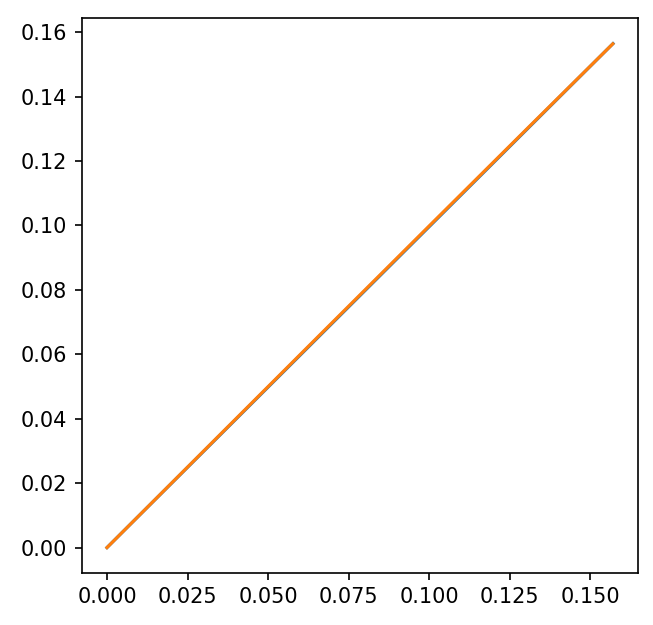
\includegraphics[width=\textwidth]{slike/usporedba40.png}
		\end{minipage}%
		\begin{minipage}{.5\textwidth}
			\centering
			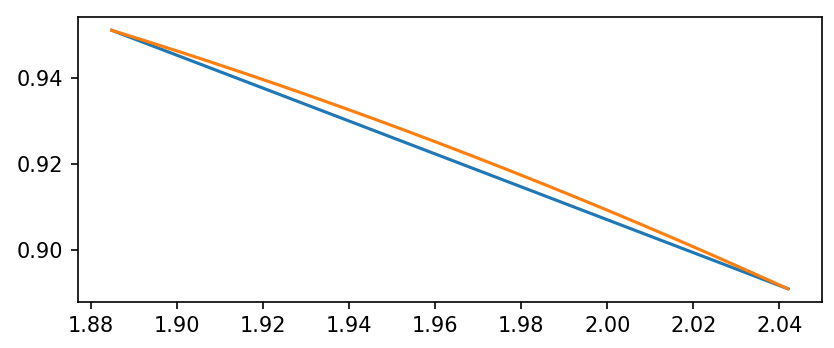
\includegraphics[width=\textwidth]{slike/usporedba412.png}
		\end{minipage}
		\caption{Usporedba funkcije $f(x)=\sin (x)$ i linearne interpolacije. Plavom bojom je prikazana interpolacija, a narančastom funkcija. Izvor: autorska izrada}
		\label{linInterSlika1}
	\end{figure}
	
\end{frame}

\begin{frame}{$f(x)=\sin x$ - kubična interpolacija}
	\begin{figure}[H]
		\centering
		\begin{tikzpicture}% function
		\begin{axis}[axis x line=center, axis y line=center, ymin=-1]
		\addplot[domain=0:2*pi,smooth, color=red] (\x,{sin(\x r)});
		\addplot[domain=0:2*pi,smooth, color=blue]
		(\x,{1*\x-((x^3)/6)});
		\end{axis}
		\end{tikzpicture}
		\caption{Prikaz funkcije $f(x)=\sin x$ (crveno) i interpolacije te funkcije polinomom trećeg stupnja $P_0(x)=1x-\frac{1}{6}x^3$ (plavo)}
	\end{figure}
\end{frame}
\section{Primjer na funkciji $g(x)=\frac{1}{x^2+1}$}
\begin{frame}{$g(x)=\frac{1}{x^2+1}$ - linearna interpolacija}
	\begin{figure}[H]
		\centering
		
		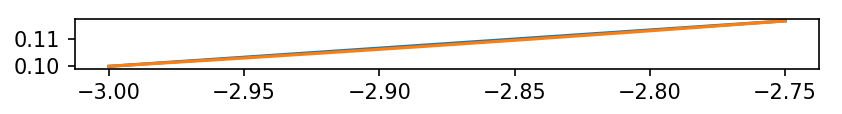
\includegraphics[width=\textwidth]{slike/usporedba58.png}
		
		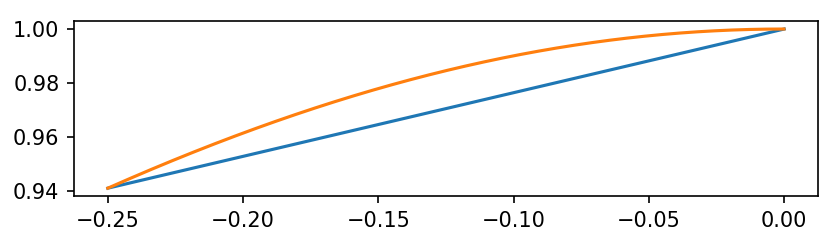
\includegraphics[width=\textwidth]{slike/usporedba519.png}
		
		\caption{Usporedba funkcije $g(x)=\frac{1}{x^2 +1}$ i linearne interpolacije za $i=9$ te $i=20$. Plavom bojom je prikazana interpolacija, a narančastom funkcija. Izvor: autorska izrada}
		\label{linInterSlika2}
	\end{figure}
\end{frame}

\begin{frame}{$g(x)=\frac{1}{x^2+1}$ - kubična interpolacija}
	\begin{figure}[H]
		\centering
		\begin{tikzpicture}% function
		\begin{axis}[
		axis x line=center, 
		axis y line=center, 
		ymin=-0.1,
		width=1\textwidth,
		height=0.6\textwidth
		%scaled ticks=false,
		]
		\addplot[domain=-5:5,smooth, color=red] (\x,{1/(\x^2+1)});
		\addplot[domain=-5:5,smooth, color=blue]
		(\x,{-2*x^2+1});
		\end{axis}
		\end{tikzpicture}
		\caption{Prikaz funkcije $g(x)=\frac{1}{x^2 +1}$ (crveno) i interpolacije te funkcije polinomom trećeg stupnja $P(x)=1-2x^2$ (plavo)}
	\end{figure}
	%\includegraphics[width=\textwidth]{slike/}
\end{frame}
\section{Zaključak}
\begin{frame}{Zaključak}
	Hvala! Pitanja?
\end{frame}
\end{document}